%
% $Id: AttributeSet.java 15 2010-10-11 16:16:32Z justinkamerman $ 
%
% $LastChangedDate: 2010-10-11 13:16:32 -0300 (Mon, 11 Oct 2010) $ 
% 
% $LastChangedBy: justinkamerman $
%

\documentclass[10pt]{report}
\usepackage{graphicx}
\usepackage{setspace}			
\onehalfspacing

\title{CS6735 Programming Assignment 1}
\author{Justin Kamerman}
\date{\today}

\begin{document}
\maketitle

%----------------------------------------
% Assignment
%----------------------------------------
\section*{Assignment}
\begin{enumerate} 
\item Implement ID3 algorithm using Java. Evaluate your implementation
  on the datasets in data.zip using 10 times 5-fold cross-validation,
  and report the average accuracy and standard deviation. All datasets
  are for UCI machine learning repository. You can check the detailed
  descriptions from the following link: 
  http://www.ics.uci.edu/~mlearn/MLRepository.html

For breast cancer data see:
http://archive.ics.uci.edu/ml/datasets/Breast+Cancer+Wisconsin+%28Diagnostic%29

For car data see:
http://archive.ics.uci.edu/ml/datasets/Car+Evaluation

For ecoli data see:http://archive.ics.uci.edu/ml/datasets/Ecoli

For letter recognition data see:
http://archive.ics.uci.edu/ml/datasets/Letter+Recognition

For mushroom data see: http://archive.ics.uci.edu/ml/datasets/Mushroom

\item Try to improve ID3 by some post pruning idea using a separate
  validation set.
\end{enumerate}

%----------------------------------------
% Submission
%----------------------------------------
\section*{Learning Algorithm}

\section*{Data Sets}

\section*{Program Design}

\begin{figure}
  \begin{center}
	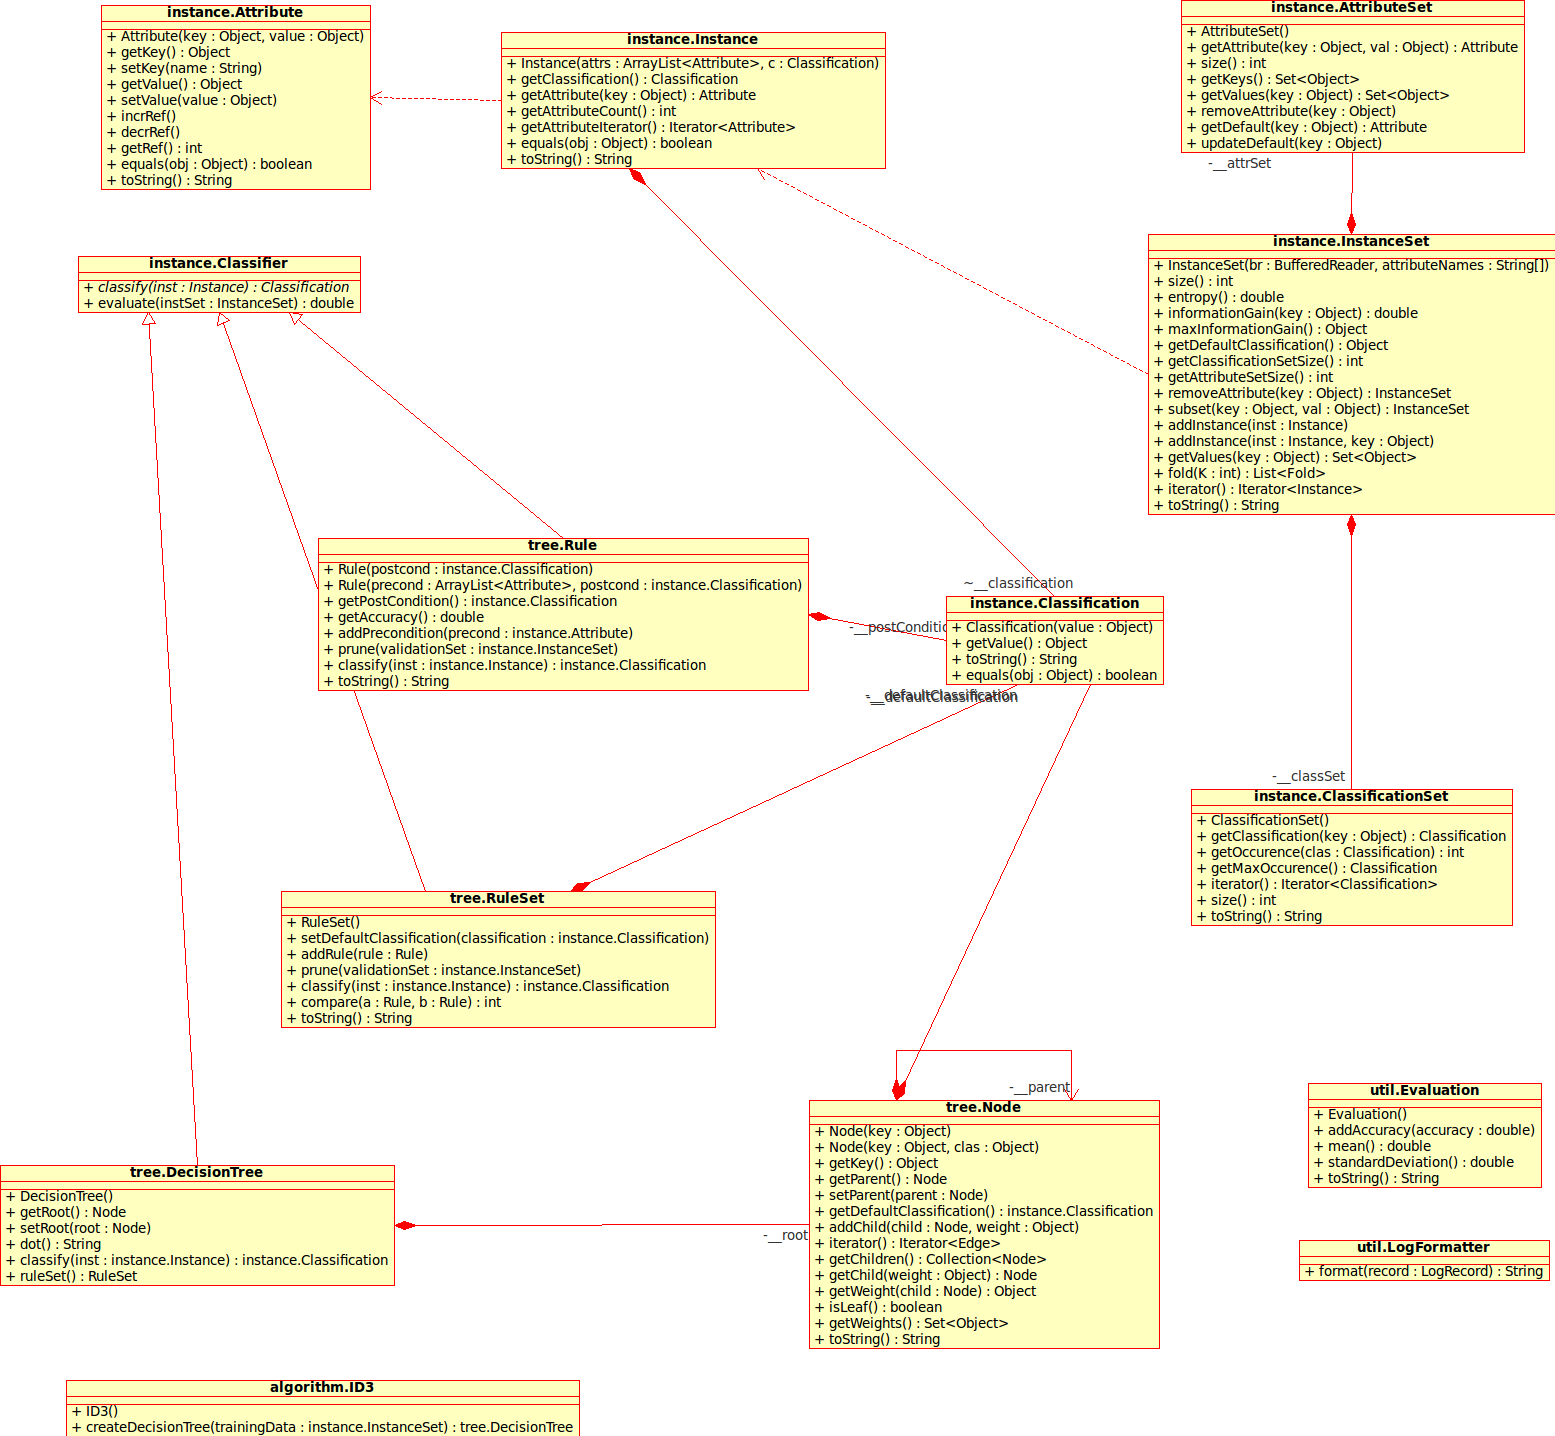
\includegraphics[angle=90,width=\textwidth,height=!]{uml}
  \end{center}
  \caption{UML class diagram}
  \label{fig:uml}
\end{figure} 


% Bibliography
%\bibliography{bibliography}
%\bibliographystyle{agsm}


%--------------------------------------------------
\end{document}
